% 2015 年重庆卷（理工农医类）第 3 题：平均气温数据的茎叶图（依固定扫描页重绘，只画拓扑与标号，不按比例）
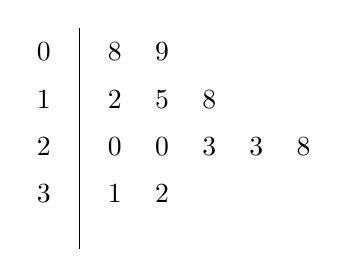
\begin{tikzpicture}[scale=1.0]
  % 茎叶分隔线
  \draw (0,2.55)--(0,-0.25);
  % 茎 0
  \node at (-0.45,2.25) {$0$};
  \node at (0.45,2.25) {$8$};
  \node at (1.05,2.25) {$9$};
  % 茎 1
  \node at (-0.45,1.65) {$1$};
  \node at (0.45,1.65) {$2$};
  \node at (1.05,1.65) {$5$};
  \node at (1.65,1.65) {$8$};
  % 茎 2
  \node at (-0.45,1.05) {$2$};
  \node at (0.45,1.05) {$0$};
  \node at (1.05,1.05) {$0$};
  \node at (1.65,1.05) {$3$};
  \node at (2.25,1.05) {$3$};
  \node at (2.85,1.05) {$8$};
  % 茎 3
  \node at (-0.45,0.45) {$3$};
  \node at (0.45,0.45) {$1$};
  \node at (1.05,0.45) {$2$};
\end{tikzpicture}
